
\let\textcircled=\pgftextcircled
\chapter{State of the art}

\initial{T}he relatively recent history of ``small'' (considered as weighting less than 25 kg) commercial UAVs implies that the technologies involved have not reached a high Technology Readiness Level (TRL) \cite{assistantsecretaryofdefenseforresearchandengineering2011} until very recently, or are still under development (TRL 6-7).
For that reason, most of the work considered in the present chapter is not yet ready for the market and has a great capacity to improve.
Universities are actively exploring the autonomous aptitudes of UAVs, but the economical exploitation potential is still small due to the low reliability issues that these systems are encountering in non-controlled environments.

In the present chapter several fields of interest to the project will be explored.
First, some environment sensing alternatives will be compared.
Then, the current commercial implementations of collision avoidance on aircraft will be studied, to finalise with ongoing research at the leading universities in UAV technology development.


\section{Environment sensing}

Knowing the environment is the initial step towards any interaction of a system with its surroundings.
That knowledge could in principle be acquired a-priori and then copied into the system, but when either time-changing or completely unknown scenarios are considered, having a means of sensing the environment is essential.

\subsection{Radar}

Radar stands for RAdio Detection And Ranging.
Its usage dates back to 1904, when H\"ulsmeyer registered the patent for his Telemobiloscope \cite{hulsmeyer1904}, using a primitive variant of the radar for detecting metallic ships.

Nowadays, the radar works by emitting one powerful radio signal impulse against the object that needs to be located.
If the signal reaches a solid object on its path, the electromagnetic wave will be distorted and part of it will be reflected back to the emission point, where a second listening antenna can detect it.

\begin{wrapfigure}{r}{0.28\textwidth}
	\centering
	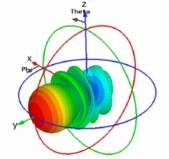
\includegraphics[width=0.25\textwidth]{./figures/antennaPattern.jpg}
	\caption{Highly directional radiation pattern. {\footnotesize Source: \url{cisco.com}}}
	\label{fig:antenna}
\end{wrapfigure}
The distance of the detected object is calculated by measuring the flight time of the signal since it was emitted until it is detected, applying the signal propagation speed ($3 \cdot 10^{^8} m/s$ for electromagnetic waves) as correction factor.
The azimuth position of the object can be estimated if the initial signal was created by a highly directional antenna, since the orientation of the transmitting antenna can be measured and the sensed object must be contained in the electromagnetic radiation field.

The fact that radar uses electromagnetic waves implies that the response time can be very high, although some technical issues may arise for the same fact at the time of processing the returned signal \cite{krolik2005}.
A more in-depth comparison of reasons for and against each of the sensing methods will be contemplated in Section \ref{sec:sensorCompare}.

\subsection{Sonar}

The ultrasonic rangefinder (commonly known as sonar, for SOund Navigation And Ranging) relies, like the radar, on the measurement of the flight time of a signal rebounding against the target.
However, instead of being electromagnetic waves, the carriers are sound waves, with a frequency usually beyond the human hearing range upper threshold (hence ultrasonic).

It is important to mention that the calculation of distance from the flight time of the rebounded signal is to some degree dependent on the environment:
The speed of propagation of sound depends on the temperature of the medium through which it propagates as $a=\sqrt{\gamma R_g T}$.
Thus, the temperature of the air should be monitored to compensate for variations during the flight.
Fortunately, the error associated with temperature changes around room temperature is of the same order than the accuracy of the sensor itself, so it is safe to consider ambient temperature at the initial calibration stage only and assume it stays constant thereafter, since it can be proven that for the measurement of distance to an object at approximately 1 metre, the error due to a temperature change of 10 K is of the order of 1 milimetre.

\subsection{Lidar}

LIght Detection and Ranging also works by measuring the time of flight of a signal.
In this case, it is a visible light pulse, usually produced by a laser for its high coherence and low dispersion.

This system is convenient for ranging objects that are small or at a long distance from the sensor, but the small measuring point of the laser beam has some limitations when the mapping of a large area is required.
In these situations, multiple measurements are usually performed sequentially with a rotation of the laser emitter between pulses, but the procedure significantly increases the latency of the system for obstacle detection, and also the complexity of the sensor system itself.

In summary, lidar is a good alternative for ranging, but not so much for detection.

\subsection{Computer vision}

The usage of regular cameras for physical environment sensing is certainly different than the previously considered, since it is not the flight time of a pulsated signal what encodes the information.
Instead, one or more cameras provide a two-dimensional array of data that can be processed to extract information of distance and location, among others, of any object that is within frame.


\subsection{Sensor comparison} \label{sec:sensorCompare}


\section{Collision avoidance}

\subsection{TCAS on conventional aircraft}

\subsection{DJI Phantom 4}

\subsection{Tesla Motors}


\section{Real-time Guidance Navigation and Control (GNC)}

\subsection{University of Pennsylvania}

\subsection{ETH Z\"urich}


